\subsection{White-box and Black-box Testing}
%basis testing
%control flow
%data flow
%AAA
We usually split testing up into two categories: black-box and white-box testing. Black-box testing refers to tests in which the tester does not have access to the source code and must hence test based on the specifications of the given methods, meaning testing based on what the method is supposed to do, hence the method works as a black-box. White-box testing is the other scenario, where the tester has access to the method. This means that the tester is aware of the control flow and routes the method can take, such that testing can rely on the inner workings of the method instead of only the specifications\cite{TestingCodeComplete}. \\
However, even though we are the developers, we do not have direct access to the code. This is because, while we do have access to the combinators and the pre-synthesised code, we will not be able to see the synthesised code during our synthesising of our tests as well. The synthesised code will work as a sort of black-box, since we do not actually know how the code looks like and hence making white-box testing would prove difficult, without analysing our generated files. So with this in mind, we have chosen to focus on black-box testing, as this seems as the more accessible and appropriate path to take. \\
Under black-box testing, we will mainly be looking at data testing. Data testing refers to the data, meaning the input of the program\cite{TestingBlackbox}. The two major methods here are equivalence partitioning and boundary conditions. Let us take a closer look on these two methods. 
\subsubsection{Equivalence Partitioning}
The most important task when it comes to testing is selecting the right test cases\cite{TestingBlackbox}. After all, if we had a simple program that took an integer as input, we could, theoretically, make infinitely many tests for this. This is where equivalence partitioning, also called equivalence classing, comes in. The idea here is that we reduce the infinite possible sets of test case, while still being as effective. We want to split the data into partitions, such that we can use a single test that counts for a range of possible input. For instance, how different would it be to test for 1, 2 and 3 as input as opposed int.MaxValue? We would expect that the first three cases would act similarly, while the program would have to handle the maximum integer value differently. However, how do we know for sure what input to put in the different partitions? The short answer is we do not. Equivalence partitioning can be subjective, such that different testers may come up with different partition sets\cite{TestingBlackbox}.
\subsubsection{Boundary Conditions}
Boundary Conditions is about testing the method at the boundaries. As a good illustration of what boundary condition is and is for, you could imagine walking along the edge of a cliff. If you can traverse this part safely, you can most likely traverse away from the edge as well. Meaning, if we can show that our methods work at the edge of their capabilities, chances are they will almost certainly work under normal conditions as well. These boundary conditions, also known as edge cases, are important since with programming, problems are more likely to occur at the edges\cite{TestingBlackbox}. This means that, for instance, if we could input any number between 1-100, it would be better to test the edges, such as 1 and 100 than numbers in the middle. \\
We can combine this with the Equivalence partitioning explained earlier. We could split our testing into two equivalence partitions. One should be the edges, those that we expect to work, meaning in our number example it could be 1 and 100. The other equivalence partition would then be outside the boundaries, meaning cases that could likely cause an error, or some unexpected behaviour. In our example, this could be 0 or -1 and 101, just outside our boundaries. 
\subsubsection{Default, Zero and Blank}
Another thing we can look at is testing our methods with a default value. In this case we mean, for instance, if our TakeDamage() method, is parsed 0, what happens then? Or the play function, which is our player's way to interact with their surroundings in the game, by entering things like "fireball witch", "go north", etc., what happens if we enter the empty string? These types of cases can be classified as forms of edge cases, but \todo{But?} they are still important to include, as these situations may have been overlooked during implementation of the methods\cite{TestingBlackbox}.
\subsubsection{AAA}
One last thing we want to look at is the structure of the individual unit tests. Usually they conform to the AAA pattern. AAA stands for arrange, act and assert. Using this form of pattern makes it easy for other people to understand your tests\cite{TestingAdaptiveCode}. \\
The arrangement part is also referred to as the setup. Before we can actually perform a certain test, we need to set up what we need in order to carry out the tests. A simple example would be instantiation of the class to be used in the test. Without instantiating the class, we will not have a valid instance to test. \\
The act part of AAA is the execution of the method to be tested. Optimally, this should only consist of a single interaction, for instance meaning a single method call\cite{TestingCodeComplete}. This ensures that the individual tests are simple and precise. \\
The last part of AAA is the assertion. This is the actual testing part, where we will see whether our act part has performed as expected, or produced another, unforeseen, outcome. \\
\\
However, we have diverged a bit from this concept for two reasons. First off, the testing framework we are using, NUnit, allows setup code to be run from the constructor. This means that the arrange aspect can partially, if not fully, be moved to the constructor of the test class. \\
The other reason is readability and transparency. If we have a test, NUnit allows the ability to run the same code with various data input. This means we can have multiple testcases, under the same test function. At a first glance, this may look better, as there is less code in the function, however, it can make the assert part more unclear. If we want to make multiple testcases of the same test, our expected value had to be dynamic, which would obfuscate what we really intended as the expected value. \\
So instead, we explicitly state what the expected outcome is. 
\begin{figure} %MINDRE?
    \centering
    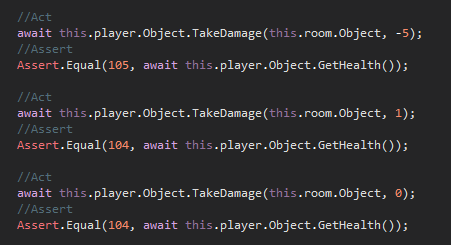
\includegraphics[width=0.8\linewidth]{Materials/TestingTheory/playerTakeDamageAAAtest}
    \caption{Part of the player's DamageTest(), showcasing the AAA structure.}
    \label{playerDamageTest}
\end{figure}
if we look at \autoref{playerDamageTest} we can see how we diverge from the described form of AAA, where our test includes the various testcases with different input, instead of feeding the data to a dynamic test. Here we can also see how we explicitly state the expected outcome for each testcase. 

% As we have been the developers of our product, we will omit black-box testing and focus on white-box testing. As stated, since white-box testing includes the source code, we can more thoroughly test our methods and hence, with white-box testing, cover the same testcases as black-box tests, making them superfluous. \\% måske?
% Now, under white-box testing we have different testing methods to make sure our tests are thorough. Futhermore, there are two aspects we will look at shortly: control-flow testing and data-flow testing. As the name suggests, control-flow testing is about testing the control statements of a method, and making sure we test all possible routes. Data-flow testing is focused on the variation of data and the idea here is that data is atleast as error-prone as control-flow and should therefore be tested as well\cite{TestingCodeComplete}. 

% \subsubsection{Structured Basis Testing}
% We will start by looking at control-flow testing. Here we have structured basis testing, which is a pretty simple concept. We want to make sure that each statement in the given method is run at least once during testing. We can use a simple approach to figuring out how many testcases are needed for basis testing at a minimum, by following these three steps\cite{TestingCodeComplete}:
% \begin{itemize}
%     \item Add a testcase for the method itself.
%     \item Add a testcase for each of the control-flow keywords in the method. (if, while, for, and, etc.)
%     \item Add a testcase for each case in a case statement. Add an additional testcase if the case statement does not include a default case.
% \end{itemize}
% For instance, if we picture a simple method that contained a simple if-statement, we would need two testcases: one for the simple path through the method, and one for the control-flow keyword if. From this we can see that, based on the complexity of the method, the number of testcases we will need to cover all statements increases quickly. \\
% So, with structured basis testing, we assure that all code of a method is executed. However, as mentioned earlier, data-flow is atleast as error-prone, and structured basis testing does not take variation of data into account.

% \subsubsection{Data-flow testing}
% With data-flow testing, we want to ensure that not only all statements are covered, but also all combinations of variables in the code. With structured basis testing, we get a weak form of data-flow testing, since this executes all lines of code, which includes all variables\cite{TestingCodeComplete}. This, in turn, gives us some of the combinations of data, but not them all. We want to extend upon the structured basis testing to include data-flow testing and this calls for more testcases. Here, we want to add all the combinations of variable states that have not been included in the structured basis testing. %Hmmmm